\chapter{Fluid Simulation}

\section{Computational Fluid Dynamics}

The study of fluid simulation is known as Computational Fluid Dynamics, which
encompasses mathematical models for fluid behavior and numerical methods for
implementing these models. The most well-known model for describing the
behavior of fluids is given by the Navier-Stokes equations. These equations
model a fluid by considering the physical quantities mass-density, pressure and
velocity as continuous fields and describing their relationships over time with
differential equations.


The numerical methods for solving these differential equations are many and
varied. These methods can usually be classified as one of two types, Eulerian
and Lagrangian. Eulerian methods describe a fluid in terms of space, while
Lagrangian methods describe a fluid in terms of material. Essentially, in an
Eulerian method one looks at a region in space and watches how much fluid moves
in and out of the region, whereas in a Lagrangian method one watches the
material properties of a small volume of fluid and tracks its movement through
space.


In general, an Eulerian method discretizes an area of space with a grid, where
each grid cell represents a small volume through which a fluid can pass. The
accuracy of Eulerian methods is largely dependent on the resolution of this
grid. Smaller cells generally imply a more accurate result but at a higher
computational expense. This presents a problem when one considers that the grid
must be stored in the limited memory of a computer, so there is a secondary
cost to making a higher resolution grid. This cost is compounded if only a
relatively small area of the grid contains fluid, since naturally one would want to
use more and smaller cells in that area and not store the unused cells in other
parts of the domain. Another related concern is when a fluid undergoes a large
deformation where additional resolution is necessary to accurately resolve the
behavior. One would then like to dynamically provide higher resolution in the area
of the deformation while leaving the rest of the grid intact.  While many
Eulerian methods address these concerns with adaptive mesh techniques, the
computational costs involved are not amenable to real-time simulations. 


Lagrangian methods naturally remove the dependence on a spatial grid since they
are based in the material description of the fluid. A common way to keep track
of the material properties of a fluid in a Lagrangian method is by using
particles, where each particle has a location in space, represents a volume of
fluid and stores material properties. Particles then interact with each other
over time, transfer material properties and are displaced according to forces
that depend on the type of fluid considered. Since the location of the
particles is not fixed, and the fluid is represented only by the particles, the
problem of limited storage is distinct from the problem of resolution. With
particle-based methods resolution is increased by adding more particles, but
without the spatial restriction.


\section{Navier-Stokes}

The Lagrangian formulation of the Navier-Stokes equation for an incompressible
isothermal viscous fluid is given by\\
1) The continuity equation:
\begin{align}
\frac{d\rho}{dt} = -\rho \grad \cdot v.
\end{align}
where $\rho$ represents the density of the fluid and $v$ represents the velocity;\\


2) The momentum equation:
\begin{align}
\frac{dv}{dt} = -\frac{1}{\rho}P + \frac{\mu}{\rho} \nabla^2 v + f.
\end{align}
where $\mu$ represents the dynamic viscosity and $f$ represents external forces (such as gravity).


\section{Smoothed Particle Hydrodynamics}


The key idea behind Smoothed Particle Hydrodynamics lies in the integral
approximation of a field function \cite{Monaghan2005}.
The integral representation of a field
function, $A$, is given by 
\begin{align}
A(r) = \int_\Omega A(r')W(r-r', h)dr'.
\end{align}

Here $r$ is a point in space, and $W$ is a kernel function with a smoothing radius
$h$, and $\Omega$ is the volume that contains $r$. If $W$ is the Dirac Delta
function, the integral representation reduces to the exact value of $A(r)$.
Otherwise it is known as a kernel approximation.

The integral representation can be discretized by a particle approximation, which is the summation of particles in a neighborhood:
\begin{align}
A(r) = \sum_j A_j V_j W(r-r_j, h).
\end{align}
where $A_j$ is the field value at coordinate $r_j$ and $V_j$ is the volume of
particle $j$. It is important to note that for a fluid, the volume of a particle is given by
its mass divided by its density:
\begin{align}
V = \frac{m}{\rho}.
\end{align}
The particle approximation of a field function in SPH is given by:
\begin{align}
    \label{eqn:sphff}
A(r) = \sum_j \frac{m_j}{\rho_j} A_j W(r - r_j, h).
\end{align} 
The gradient of a field function is given by:
\begin{align}
\nabla A(r) = \sum_j \frac{m_j}{\rho_j} A_j \nabla W(r - r_j, h).
\end{align}
Since $A_j$ is assumed constant in the volume $V_j$, only the kernel function
$W$ is affected by the gradient. Similarly the Laplacian of a field function is
given by
\begin{align}
\nabla^2 A(r) = \sum_j \frac{m_j}{\rho_j} A_j \nabla^2 W(r - r_j, h).
\end{align}


\subsection{Formulation}

Applying the SPH approximations to the Lagrangian formulation of the
Navier-Stokes equations is done in two steps. By keeping the mass fixed for each
particle the continuity equation can be omitted, instead the density of each particle is approximated:
\begin{align}
\rho_i = \sum_j \rho_j \frac{m_j}{\rho_j} W(r_i - r_j, h)
\end{align}
using equation \ref{eqn:sphff} which can be simplified to
\begin{align}
\rho_i = \sum_j m_j W(r_i - r_j, h).
\end{align}
\\
\\
The momentum equation
\begin{align}
\frac{dv}{dt} = -\frac{1}{\rho}P + \frac{\mu}{\rho} \nabla^2 v + f
\end{align}
can be separated into three components on the right hand side:
\begin{align} \frac{dv}{dt} = F^{pressure} + F^{viscosity} + f^{external} \end{align}
with
\begin{align}
F^{pressure} = -\frac{1}{\rho}P
\end{align}
and
\begin{align}
F^{viscosity} = \frac{\mu}{\rho} \nabla^2 v.
\end{align}
To approximate the pressure force, an equation of state is used to give weak
compressibility, rather than solve the Poisson pressure equation for near
incompressibility, to reduce computational cost.
The equation of state is given as 
\begin{align}
P = k(\rho - \rho_0)
\end{align}
Where $k$ is a gas stiffness constant and $\rho_0$ is the rest density.
The pressure term can be approximated as
\begin{align}
F^{pressure}_i = -\frac{1}{\rho_i} \sum_j P_j \frac{m_j}{\rho_j} \nabla W(r_i - r_j, h).
\end{align}
However this does not produce a symmetric force and violates the action-reaction law. A symmetric approximation of the gradient is used instead:
\begin{align}
F^{pressure}_i = -\frac{1}{\rho_i} \sum_j \frac{P_i + P_j}{2} \frac{m_j}{\rho_j} \nabla W(r_i - r_j, h).
\end{align}
The SPH formulation of the viscosity term is given as follows
\begin{align}
F^{viscosity}_i = \frac{\mu}{\rho_i} \sum_j (v_j - v_i) \frac{m_j}{\rho_j} \nabla^2 W(r_i - r_j, h).
\end{align}


\subsection{Kernel Functions}

The kernel functions used in the integral representations have a large impact
on the accuracy and consistency of the method. Kernel functions and their
derivatives must have compact support, having a value of 0 outside of the
smoothing radius. The behavior of the kernel functions and their derivatives
can also strongly impact the behavior of the particles, so care is taken when
selecting a kernel \cite{Liu2010}.

The following kernels were selected for their performance in \cite{Krog2010}.
\\
For density approximation the $W_{poly6}$ kernel is used
\begin{align}
W_{poly6}(r, h) = \frac{315}{64 \pi h^9} 
\begin{cases}
    (h^2 - |r|^2)^3 & \text{$0 \le |r| \le h$}
    \\
    0 & \text{$otherwise$}.
\end{cases}
\end{align}

For the pressure term the gradient of the  $W_{spiky}$ kernel is used
\begin{align}
W_{spiky}(r, h) = \frac{15}{\pi h^6} 
\begin{cases}
    (h - |r|)^3 & \text{$0 \le |r| \le h$}
    \\
    0 & \text{$otherwise$}
\end{cases}
\end{align}
with the gradient given by
\begin{align}
\nabla W_{spiky}(r, h) = -\frac{45}{\pi h^6} \frac{r}{|r|}
\begin{cases}
    (h - |r|)^2 & \text{$0 \le |r| \le h$}
    \\
    0 & \text{$otherwise$}.
\end{cases}
\end{align}

For the viscosity term the Laplacian of the $W_{viscosity}$ kernel is used
$W_{viscosity}$   
\begin{align}
W_{viscosity}(r, h) = \frac{315}{2 \pi h^3} 
\begin{cases}
    -\frac{|r|^3}{2h^3} + \frac{|r|^2}{h^2} + \frac{h}{2|r|} - 1 & \text{$0 \le |r| \le h$}
    \\
    0 & \text{$otherwise$}
\end{cases}
\end{align}
with the Laplacian given by
\begin{align}
\nabla^2 W_{viscosity}(r, h) = \frac{45}{\pi h^6}
\begin{cases}
    h - |r| & \text{$0 \le |r| \le h$}
    \\
    0 & \text{$otherwise$}.
\end{cases}
\end{align}

\begin{figure}[!htc]
 		\centering
		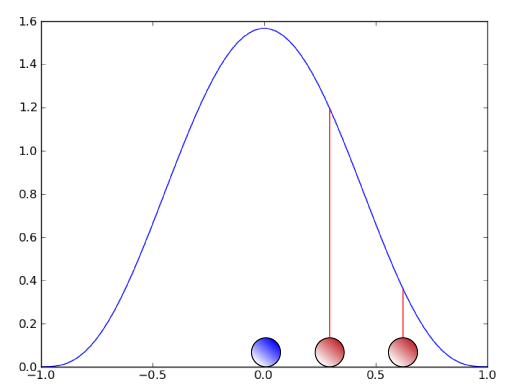
\includegraphics[scale=0.6]{figures/poly6kernel.png}
        \caption{ $W_{poly6}$ kernel in 1 dimension }
		\label{fig:poly6kernel}
\end{figure}


\subsection{Collisions}

Collisions are handled by exerting a repulsion force on particles which collide
with a surface. The repulsion force is given by
\begin{align}
F^{repulsion} = (stiffness * distance - dampening * n \cdot v))*n;
\end{align}
where $n$ is the normal of the surface, $v$ is the velocity of the particle,
$distance$ is the distance of the particle to the surface and
$stiffness$ and $dampening$ are user-defined parameters to control the behavior of
the repulsion force.\cite{Krog2010}

\subsubsection{Domain}
For convenience the fluid is considered to exist in a domain, where each wall
of the domain is a surface against which the particles can collide. The walls
are defined as minimum or maximum values in each axis, with a corresponding
normal along the axis pointing inside the domain. 

\subsubsection{Triangles}

Collisions with arbitrary triangles are calculated are performed by using an
algorithm for intersecting a line segment with a triangle from \cite{Ericson}. The line segment is
created by adding the velocity scaled by a distance parameter to the particle
position. The technique uses barycentric coordinates to test if the point where
the segment intersects with the plane of the triangle is within the triangle.
The implemented routine is given in Appendix X.

%\cite{Ericson} %Real-Time collision detection pp 191


\section{Integration}

The SPH method provides the forces which describe the change in velocity over
time. Two modifications are made to these forces to increase stability. The
first is a speed limit, which clamps the magnitude of the force to a user defined speed.
\begin{align}
F = \begin{cases} s * \frac{F}{|F|} & \text{if $|F| > s$}
    \\
    F & \text{$otherwise$}
\end{cases}
\end{align}
where $s$ is the user defined speed limit and $F$ is the force vector.

The second modification is a smoothing of the velocity given by
\begin{align}
v_i = v_i + \epsilon \sum_{j \ne i} 2m_j \frac{(v_j - v_i)}{(\rho_i + \rho_j)} W(r_i - r_j, h)
\end{align}
where $\epsilon$ is a user defined parameter between $0$ and $1$.

\subsection{Time Integration}
To advect the particles in time, the second order Leap-Frog integration method
is used. The new position and velocity each time step is given by
\begin{align}
x_{i+1} = x_i + v_i dt + \frac{a_i}{2} dt^2
\end{align}
\begin{align}
v_{i+1} = v_i + \frac{(a_i + a_i+1)}{2} dt
\end{align}
where $i$ denotes the current time-step, $x$ is the position vector, $v$ is the velocity vector and $a$ is the acceleration vector.

